\documentclass{standalone}
\usepackage{tikz}
\usepackage{ctex,siunitx}
\setCJKmainfont{Noto Serif CJK SC}
\usepackage{tkz-euclide}
\usepackage{amsmath}
\usepackage{wasysym}
\usetikzlibrary{patterns, calc}
\usetikzlibrary {decorations.pathmorphing, decorations.pathreplacing, decorations.shapes}
\begin{document}
\small
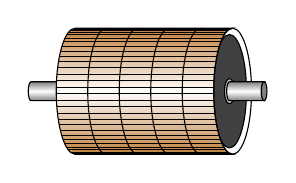
\begin{tikzpicture}[>=latex,scale=0.8]
  % \useasboundingbox(0.9,0)rectangle(5.1,5);
  \draw[top color=gray,bottom color=gray,middle color=white](-0.7,0.15)arc(90:270:0.045 and 0.15)--(1,-.15)arc(270:90:0.045 and 0.15)--cycle;
  \draw[fill=darkgray](2.45,0)ellipse(0.27 and 0.9);
  \draw[top color=brown,bottom color=brown,middle color=white](0,1)arc(90:270:0.3 and 1.0)--(2.5,-1)arc(270:90:0.3 and 1.0)--cycle;
  \draw(2.5,0)ellipse(0.3 and 1.0);
  \draw[fill=lightgray](2.45,0)ellipse(0.08 and 0.2);
  \draw[top color=gray,bottom color=gray,middle color=white](2.45,0.15)arc(90:270:0.045 and 0.15)--(3.0,-.15)arc(270:90:0.045 and 0.15)--cycle;
  \draw[fill=gray](3.0,0)ellipse(0.045 and 0.15);
  \foreach \x in {90,96,...,270}
  {
    \draw[line width=0.05mm]({0.3*cos(\x+2)},{sin(\x+2)})--++(2.5,0);
  }
  \foreach \x in {0.5,1,1.5,2}
  {
    \draw(\x,1)arc(90:270:0.3 and 1.0);
  }
\end{tikzpicture}
\end{document}